

\section{Student Module Implementation}
After successful authentication, students are directed to their application portal. The primary task for a student is to complete the comprehensive admission form, providing accurate personal and academic information.

\subsection{Final Admission Form}
The admission form is designed to collect detailed geographical and identification data. To ensure data integrity, the system implements strict front-end validation for each input field.

\begin{figure}[htbp]
    \centering
    % Ensure your file is at this exact path: chapters/chapter4/images/form.png
    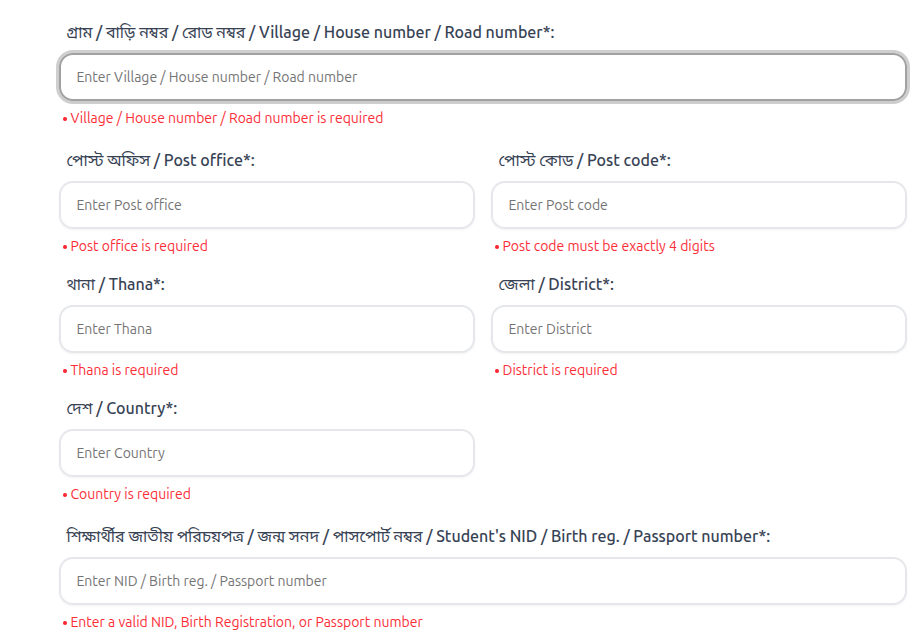
\includegraphics[width=0.85\textwidth]{chapters/chapter4/images/form.png}
    \caption{Student Admission Form with Validation}
    \label{fig:student_form}
\end{figure}

As shown in Figure \ref{fig:student_form}, the form focuses on the following components:

\begin{itemize}
    \item \textbf{Address Details:} The form requires the student's \textit{Village/House number}, \textit{Post Office}, \textit{Thana}, \textit{District}, and \textit{Country}. Each field is marked with an asterisk (*), indicating it is mandatory.
    \item \textbf{Postal Code Validation:} A specific validation rule is applied to the \textbf{Post Code} field, requiring exactly 4 digits, which prevents incorrect data entry.
    \item \textbf{Identification Information:} The system provides a flexible identification section where students must enter either their \textbf{NID}, \textbf{Birth Registration}, or \textbf{Passport number}.
    \item \textbf{Real-time Error Handling:} As illustrated in the figure, the system uses reactive validation. If a user leaves a field empty or enters invalid data (e.g., an incomplete post code), a red error message appears immediately below the input field to guide the user.
    \item \textbf{Bilingual Interface:} Continuing the design philosophy, all labels are provided in both Bengali and English to ensure clarity for all applicants.
\end{itemize}

This structured approach ensures that the database receives clean, formatted data, which simplifies the subsequent verification process by the Dean and Registrar offices.